\subsection{K-Means Clustering}

For the application of the K-means clustering, a suitable choice for the hyperparameter $K$ - the desired number of clusters - has to be found. In order to do so, Fig.~\ref{fig:G_vs_K} reports the total within-cluster variation $G$ as a function of the number of clusters $K$. A decrease of the total within-cluster variation $G$ means that the words in each cluster become more similar. However, the within-cluster variation $G$ is a strictly decreasing function of $K$. Thus, a smaller $G$ does not necessarily mean that the clustering is more accurate as a larger $K$ leads \textit{always} to a smaller $G$. A reasonable tradeoff is to chose $K$ such that the decrease of $G$ as a function of the cluster number $K$ has already become small. In other words, $K$ is taken in an interval where the total within-cluster variation decreases only slightly in comparison to its initial decrease for small values of $K$. Usually, this method is called ellbow method as the most suitable value of $K$ lies in an ellbow-shaped part of the curve. In the present case, the value $K=8$ - indicated by the dashed, red line in the Figure - marks a point in such an ellbow, and is used for further analyses.

\begin{figure}[h!]
\centering
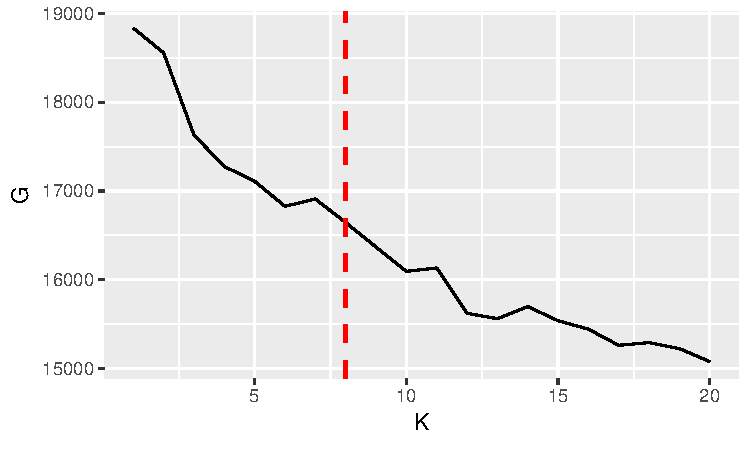
\includegraphics[width=0.8\textwidth]{G_vs_K.pdf}
\caption{Total within-cluster variation $G$ as a function of the number of clusters $K$ using K-means clustering. The dashed, red line indicates the value $K=8$ which is used for the further analysis based on the ellbow method, see the main text for more details. The most common Tweeted words in the $K=8$ clusters are reported in Fig.~\ref{fig:K_cluster}, while the number of Tweets in each cluster is summarized in Tab.~\ref{tab:tweets_per_cluster}.}
\label{fig:G_vs_K}
\end{figure}

If the desired number of clusters is set to $K=8$, the Tweets are distributed among the clusters as reported in Tab.~\ref{tab:tweets_per_cluster}. Most remarkably is cluster $3$ with $9693$ associated Tweets. Note that the numbering of the clusters is arbitrary, and does not indicate any hierarchy among the clusters.

\begin{table}[h!]
\centering
\begin{tabular}{c||c|c|c|c|c|c|c|c} 
cluster & $1$ & $2$ &$3$ &$4$ &$5$ &$6$ &$7$ &$8$ \\
 \hline
\# Tweets & $154$ & $831$ &$9693$ &$128$ &$113$ &$413$ &$102$ &$283$
\end{tabular}
\caption{Number of Tweets per cluster for the application of K-means clustering with $K=8$ clusters. The total number of tweets is $11717$.}
\label{tab:tweets_per_cluster}
\end{table}

Fig.~\ref{fig:K_cluster} shows the $10$ most common words in the Tweets in each of the $K=8$ clusters. The numbering of the clusters is the same as in Tab.~\ref{tab:tweets_per_cluster}. \\

Cluster $3$ mainly contains positive emotions like \enquote{good}, \enquote{great}, and \enquote{yeah}. These are connected to the term \enquote{model}. There is also the word \enquote{coming}. A summary of cluster $3$ could be Elon Musk's euphoria towards a \enquote{coming model}. 

Cluster $2$ and cluster $8$ give insight in what is meant with the term \enquote{model}. Both clusters show a connection with the word \enquote{tesla}. Especially cluster $8$ reveals that the term \enquote{model} refers to a new \enquote{car}. Additionally, the \enquote{electric} car might have an \enquote{autopilot}. 

Cluster $7$ includes mostly energy-related terms such as \enquote{solar}, \enquote{power}, and \enquote{battery}. Here, also the term \enquote{tesla} - that is related to cars - occurs. 

The clusters $1$, $4$, and $6$ are related to rockets and space. In cluster $1$, especially the planet \enquote{mars} appears to be of interest to Elon Musk. Cluster $4$ reveals that \enquote{raptor} might be the name of a rocket \enquote{engine}. In general, the terms \enquote{falcon} and \enquote{starship} seem to be related to rockets though it is not clear what they specifically describe.

\begin{figure}[h!]
\centering
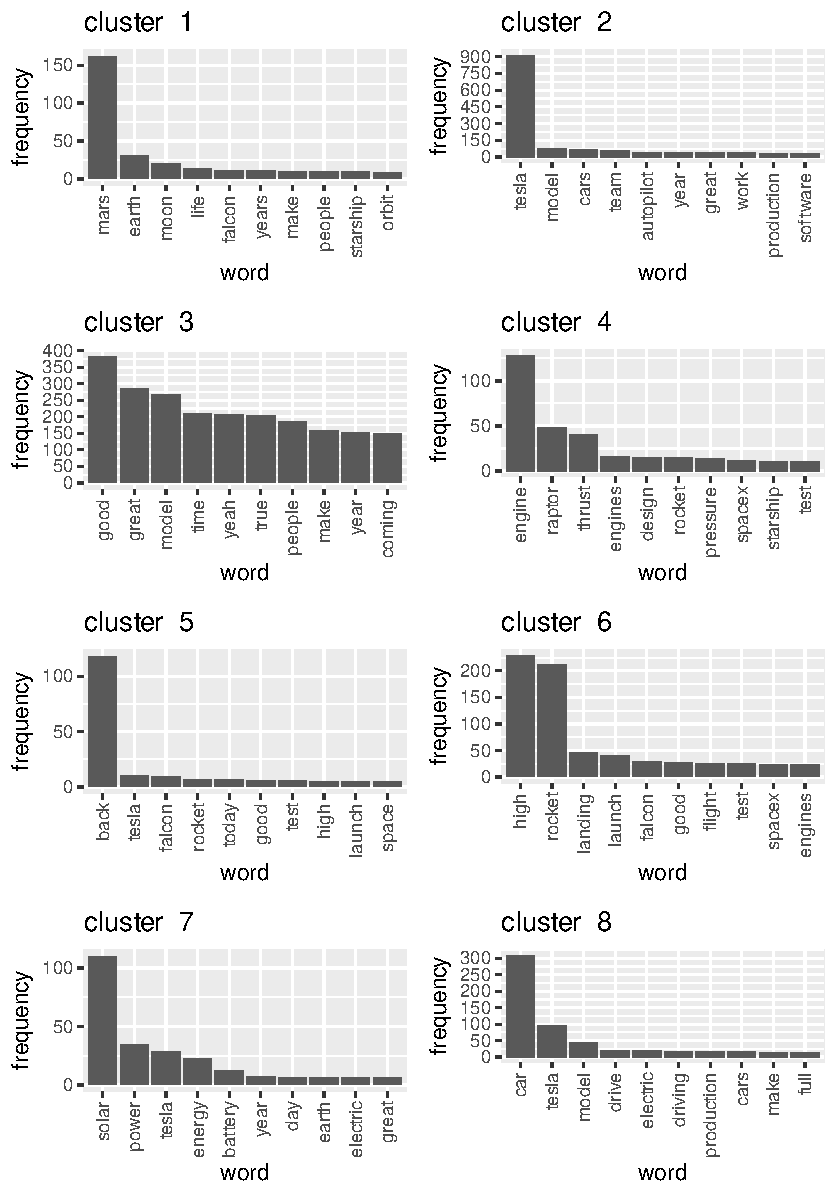
\includegraphics[width=0.8\textwidth]{K_cluster.pdf}
\caption{Barplot of the $10$ most common Tweeted words in $K=8$ clusters using K-means clustering. The meaning of the clusters in detail is discussed in the main text.}
\label{fig:K_cluster}
\end{figure}

\subsection{Hierarchical Clustering}

In contrast to the K-means clustering from the last Subsection, the hierarchical clustering does not require an a priori selection of the desired number of groups. However, as explained in the theory Section, a distance measure between the words as well as the linkage as a measure of dissimilarity between clusters has to be defined. In the present work, the binary distance (also called Jaccard distance) in combination with Ward's minimum variance method as the linkage are found to lead to the most interpretable clustering results. Note that Ward's minimum variance method is originally designed to be combined with the Euclidean distance. Nonetheless, given the excellent results of the combination with the binary distance, this combination is underlies the following discussion of the hierarchical clustering.\\

Fig.~\ref{fig:hclust_dendogram} shows the so-called dendogram of the application of the hierarchical clustering to the $140$ words of the term-document matrix. Each leaf of the dendogram is one word. The dendogram reports how the single words are merged to clusters, and how these clusters are fused to larger clusters. The root of the dendogram is a cluster that contains all words. The vertical axis at the lefthand side of the dendogram shows the value of the dissimilarity measure (in this case Ward's minimum variance method in combination with the binary distance) at the respective height of the dendogram. Clusters that are merged at a lower height are more similar than clusters that are merged at a higher point of the dendogram. 

\begin{sidewaysfigure}
    \centering
    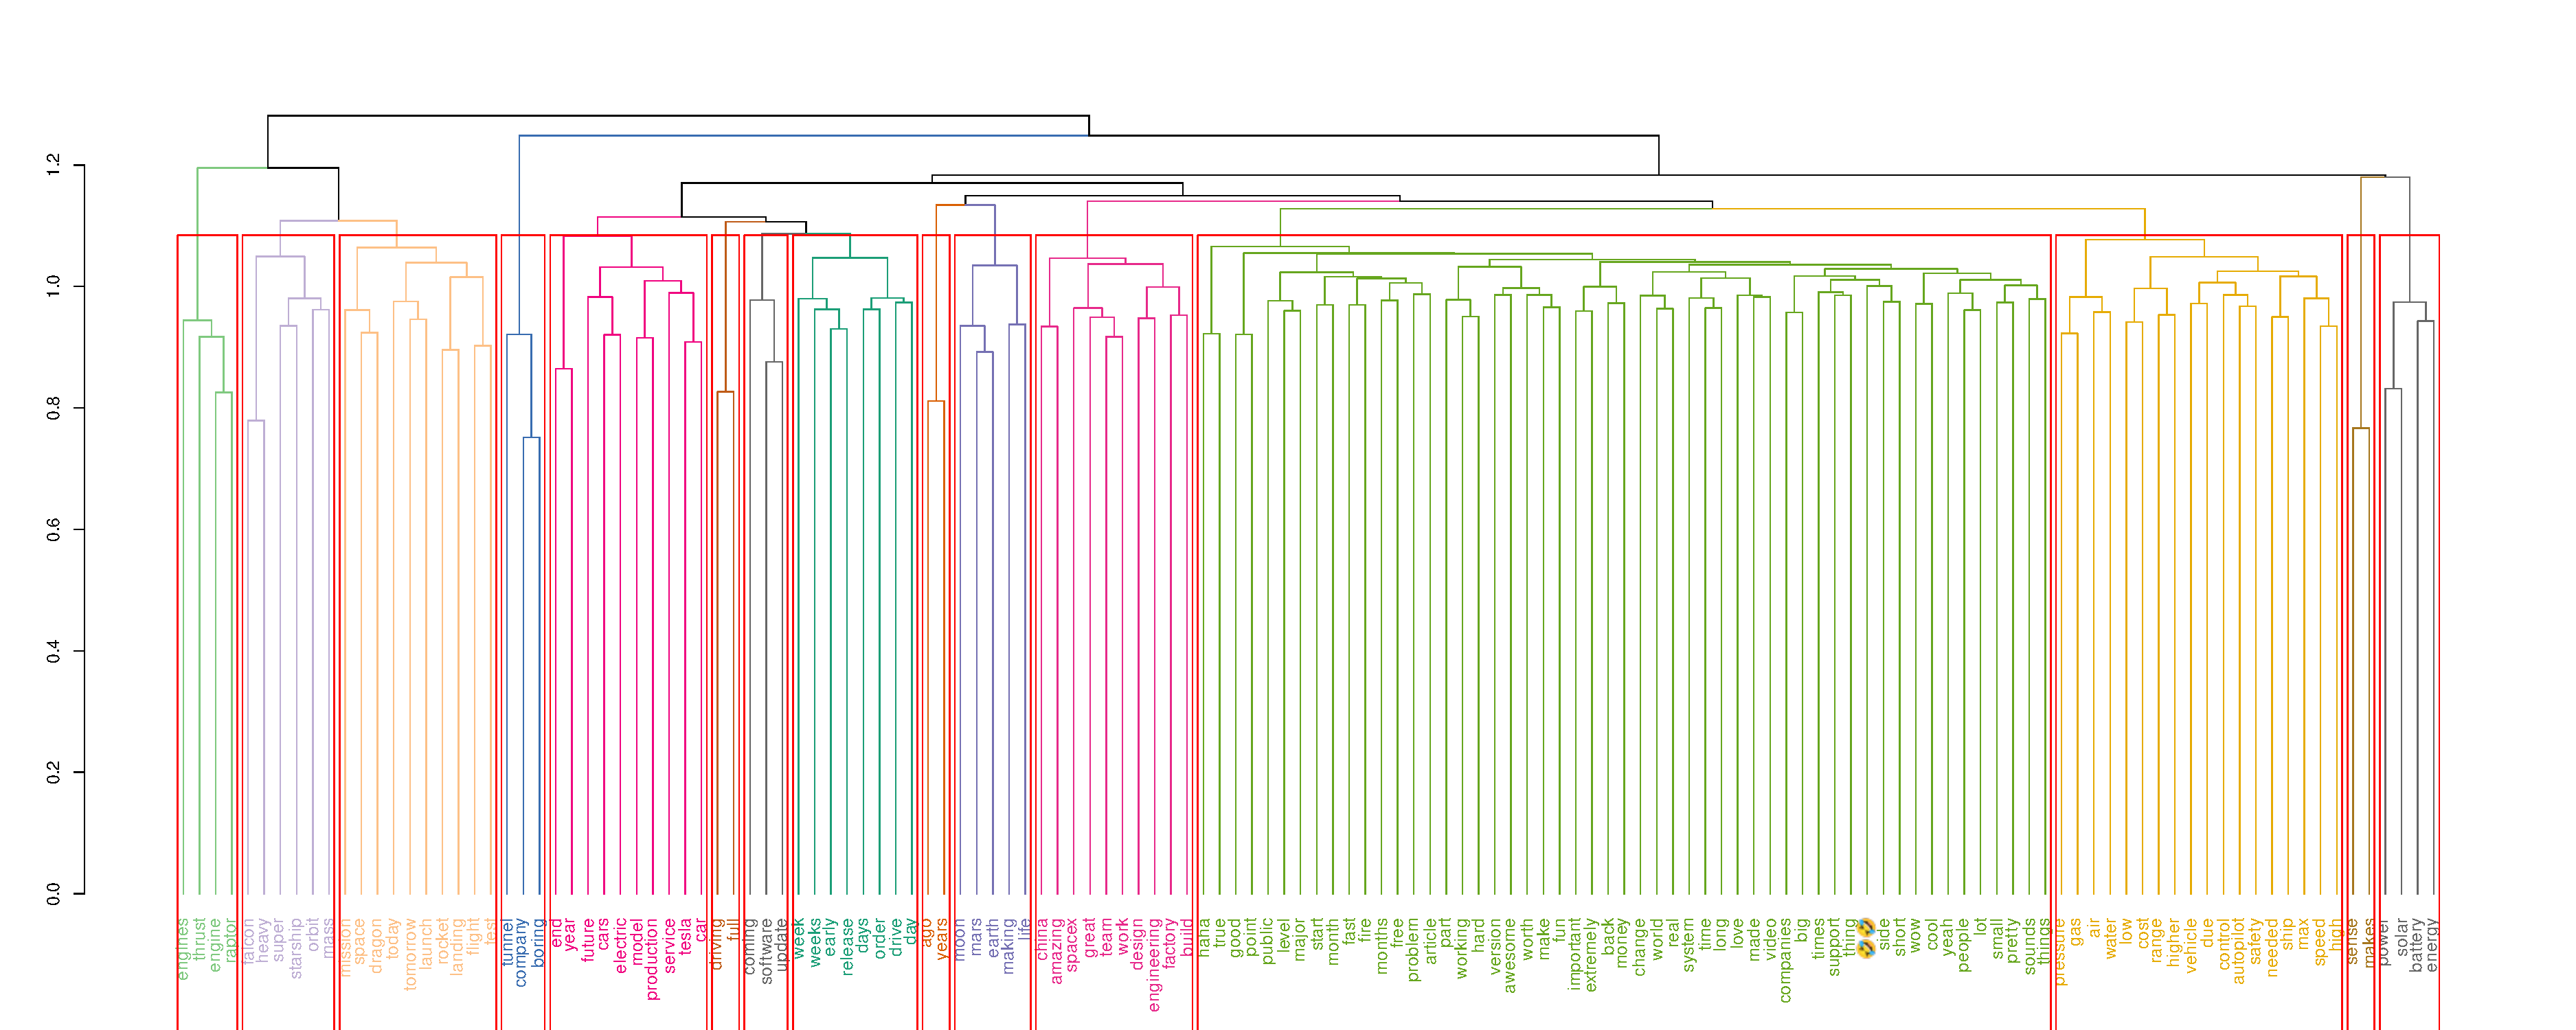
\includegraphics[width=\textwidth]{hclust_dendogram.pdf}
    \caption{Dendogram for the application of hierarchical clustering on the $140$ words of the term-document matrix of Elon Musk's Tweets. The vertical axis shows the value of the dissimilarity measure (in this case Ward's minimum variance method in combination with the binary distance) at the respective height. The red boxes and colorization of the different parts of the dendogram show the word categorization for $15$ clusters. A visualization of the words in the $15$ clusters is given in Fig.~\ref{fig:hclust_wordclouds}.}
    \label{fig:hclust_dendogram}
\end{sidewaysfigure}

\begin{sidewaysfigure}
    \centering
    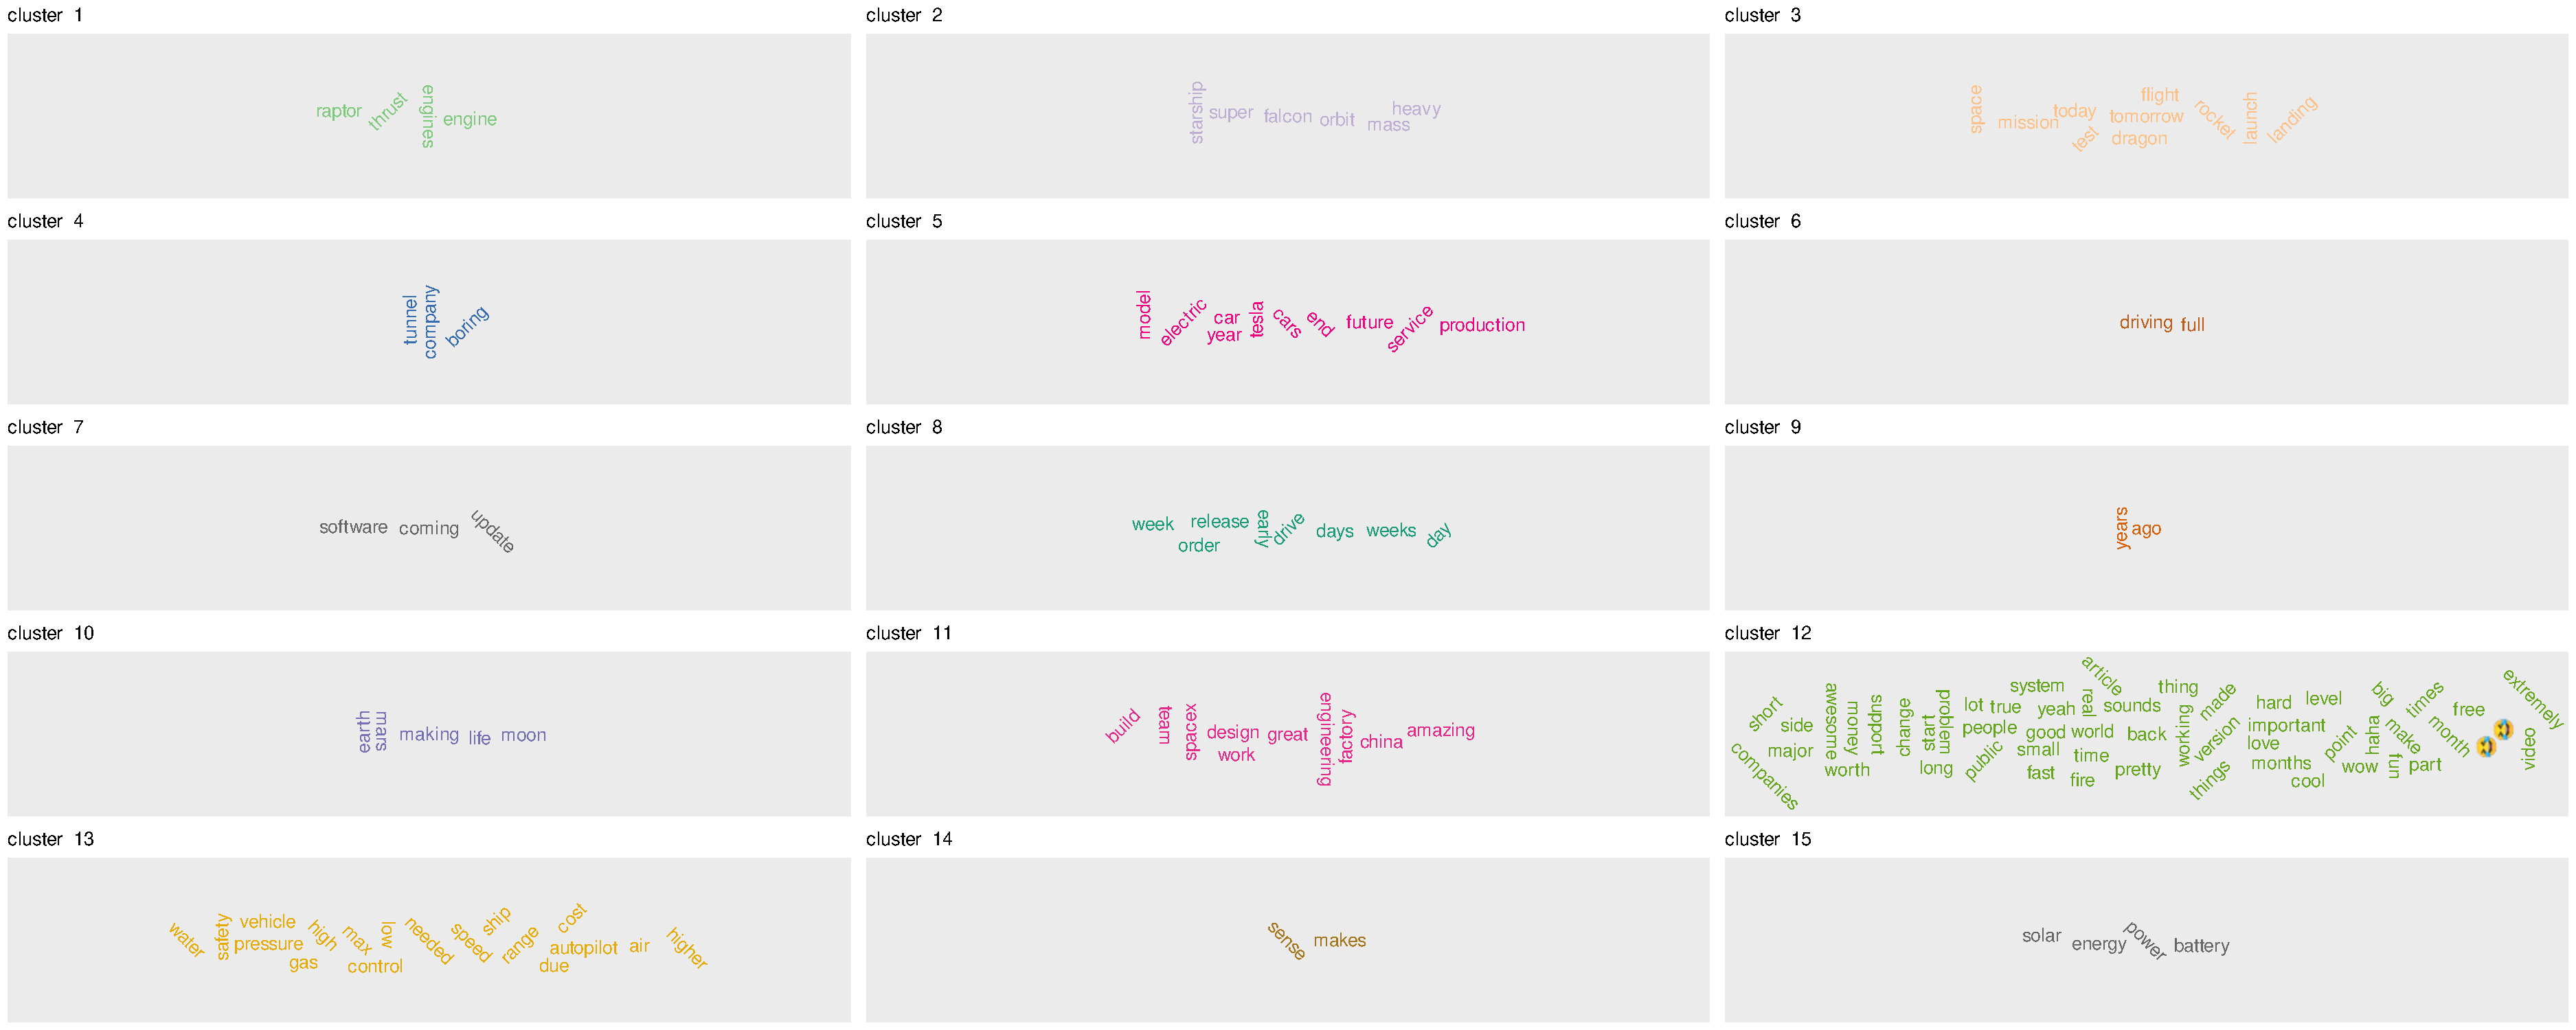
\includegraphics[width=\textwidth]{hclust_wordclouds.pdf}
    \caption{Wordclouds of the $15$ clusters obtained from the application of hierarchical clustering in Fig.~\ref{fig:hclust_dendogram}. An interpretation of the clusters can be found in the main text.}
    \label{fig:hclust_wordclouds}
\end{sidewaysfigure}
